% Options for packages loaded elsewhere
\PassOptionsToPackage{unicode}{hyperref}
\PassOptionsToPackage{hyphens}{url}
%
\documentclass[
  hyperref, a4paper]{ctexart}
\usepackage{lmodern}
\usepackage{amssymb,amsmath}
\usepackage{ifxetex,ifluatex}
\ifnum 0\ifxetex 1\fi\ifluatex 1\fi=0 % if pdftex
  \usepackage[T1]{fontenc}
  \usepackage[utf8]{inputenc}
  \usepackage{textcomp} % provide euro and other symbols
\else % if luatex or xetex
  \usepackage{unicode-math}
  \defaultfontfeatures{Scale=MatchLowercase}
  \defaultfontfeatures[\rmfamily]{Ligatures=TeX,Scale=1}
\fi
% Use upquote if available, for straight quotes in verbatim environments
\IfFileExists{upquote.sty}{\usepackage{upquote}}{}
\IfFileExists{microtype.sty}{% use microtype if available
  \usepackage[]{microtype}
  \UseMicrotypeSet[protrusion]{basicmath} % disable protrusion for tt fonts
}{}
\makeatletter
\@ifundefined{KOMAClassName}{% if non-KOMA class
  \IfFileExists{parskip.sty}{%
    \usepackage{parskip}
  }{% else
    \setlength{\parindent}{0pt}
    \setlength{\parskip}{6pt plus 2pt minus 1pt}}
}{% if KOMA class
  \KOMAoptions{parskip=half}}
\makeatother
\usepackage{xcolor}
\IfFileExists{xurl.sty}{\usepackage{xurl}}{} % add URL line breaks if available
\IfFileExists{bookmark.sty}{\usepackage{bookmark}}{\usepackage{hyperref}}
\hypersetup{
  pdftitle={ 项目时间计划书},
  pdfauthor={Shi, Ruixin; Zhang, Cenyuan; Zhang, Yihan; Wang, Chen; Zhang, Hongnian; Song, Puqi; Huang, Huiru; Tian, Ziwei},
  hidelinks,
  pdfcreator={LaTeX via pandoc}}
\urlstyle{same} % disable monospaced font for URLs
\usepackage{graphicx,grffile}
\makeatletter
\def\maxwidth{\ifdim\Gin@nat@width>\linewidth\linewidth\else\Gin@nat@width\fi}
\def\maxheight{\ifdim\Gin@nat@height>\textheight\textheight\else\Gin@nat@height\fi}
\makeatother
% Scale images if necessary, so that they will not overflow the page
% margins by default, and it is still possible to overwrite the defaults
% using explicit options in \includegraphics[width, height, ...]{}
\setkeys{Gin}{width=\maxwidth,height=\maxheight,keepaspectratio}
% Set default figure placement to htbp
\makeatletter
\def\fps@figure{htbp}
\makeatother
\setlength{\emergencystretch}{3em} % prevent overfull lines
\providecommand{\tightlist}{%
  \setlength{\itemsep}{0pt}\setlength{\parskip}{0pt}}
\setcounter{secnumdepth}{5}
\usepackage{array}
\usepackage{amsmath}
\usepackage{multirow}
\usepackage{float}

\title{\vspace{2in} 项目时间计划书}
\usepackage{etoolbox}
\makeatletter
\providecommand{\subtitle}[1]{% add subtitle to \maketitle
  \apptocmd{\@title}{\par {\large #1 \par}}{}{}
}
\makeatother
\subtitle{FaceGen: A face image generator website based on GAN}
\author{Shi, Ruixin\footnote{Equal Contribution, Fudan University, 17302010065
  (\href{mailto:rxshi17@fudan.edu.cn}{\nolinkurl{rxshi17@fudan.edu.cn}})} \and Zhang, Cenyuan\footnote{Equal Contribution, Fudan University,
  17302010068
  (\href{mailto:cenyuanzhang17@fudan.edu.cn}{\nolinkurl{cenyuanzhang17@fudan.edu.cn}})} \and Zhang, Yihan\footnote{Equal Contribution, Fudan University, 17302010076
  (\href{mailto:zhangyihan17@fudan.edu.cn}{\nolinkurl{zhangyihan17@fudan.edu.cn}})} \and Wang, Chen\footnote{Equal Contribution, Fudan University, 16307110064
  (\href{mailto:wangc16@fudan.edu.cn}{\nolinkurl{wangc16@fudan.edu.cn}})} \and Zhang, Hongnian\footnote{Equal Contribution, Fudan University,
  17302010061
  (\href{mailto:17302010061@fudan.edu.cn}{\nolinkurl{17302010061@fudan.edu.cn}})} \and Song, Puqi\footnote{Equal Contribution, Fudan University, 17302010037
  (\href{mailto:17302010037@fudan.edu.cn}{\nolinkurl{17302010037@fudan.edu.cn}})} \and Huang, Huiru\footnote{Equal Contribution, Fudan University, 17302010080
  (\href{mailto:17302010080@fudan.edu.cn}{\nolinkurl{17302010080@fudan.edu.cn}})} \and Tian, Ziwei\footnote{Equal Contribution, Fudan University, 17302010071
  (\href{mailto:17302010071@fudan.edu.cn}{\nolinkurl{17302010071@fudan.edu.cn}})}}
\date{2020年11月10日}

\begin{document}
\maketitle

\newpage

\LARGE

\begin{center}
\textbf{项目管理计划书}
\end{center}

\large
\begin{center}
\textbf{\emph{FaceGen: A face image generator website based on GAN}}
\end{center}

\hypertarget{ux9879ux76eeux63cfux8ff0}{%
\section{项目描述}\label{ux9879ux76eeux63cfux8ff0}}

随着互联网的发展,各种应用的出现,人们对塑造个性化的虚拟形象、定制具有某些特征的头像的需求也随之增多,生成的头像可以用于各类应用中,人脸生成这一项任务应运而生。
针对人脸生成任务,我们在项目中将使用TensorFlow搭建一个生成式对抗网络模型,并采用LSUN数据集,ImageNet1k和celebA数据集来对模型进行训练,最终得到能够产生人脸的图像的生成器。并且,在训练好的模型的基础上,我们将会完成一个前端网页,以可视化输入生成器的噪声向量并方便用户调整输入,以及在网页上展示生成器最终生成的图像。

\hypertarget{ux9879ux76eeux5206ux89e3}{%
\subsection{项目分解}\label{ux9879ux76eeux5206ux89e3}}

见表1

\begin{table}
    \caption{项目进度计划}
    \centering
    \begin{tabular}{|p{2.0cm}<{\centering}|p{1.0cm}<{\centering}|p{2.0cm}<{\centering}|p{2.0cm}<{\centering}|p{2.0cm}<{\centering}|}
    \hline
    任务名称     & 耗时(天) & 开始         & 结束         \\ \hline
    \textbf{DCGAN}    & \textbf{76}    & \textbf{2020-9-26}  & \textbf{2020-12-11} \\ \hline
    项目分析     & 5     & 2020-9-26  & 2020-9-31  \\ \hline
    搭建模型     & 18     & 2020-10-9  & 2020-10-27 \\ \hline
    获取与处理数据集 & 26     & 2020-10-15 & 2020-11-10 \\ \hline
    实现Demo   & 31    & 2020-11-10 & 2020-12-11 \\ \hline
    \end{tabular}
\end{table}

\hypertarget{ux5de5ux4f5cux63cfux8ff0}{%
\subsection{工作描述}\label{ux5de5ux4f5cux63cfux8ff0}}

见表2

\begin{table}
    \caption{任务描述}
    \centering
    \begin{tabular}{|p{5.0cm}<{\centering}|p{7.5cm}<{\centering}|}
    \hline
    任务       & 补充说明                                                 \\ \hline
    搭建生成模型   & 使用TensorFlow搭建DCGAN的生成器                             \\ \hline
    搭建判别模型   & 使用TensorFlow搭建DCGAN的判别器                              \\ \hline
    直接获取数据集  & 训练使用的数据集包括LSUN数据集,ImageNet 1k和celebA数据集             \\ \hline
    构造数据集    & 爬取网上社区的图片,通过openface进行修剪来构造数据集                      \\ \hline
    预处理数据集   & 调整图像大小,进行图像标准化处理                                    \\ \hline
    训练模型     & 通过优化目标函数训练模型                                        \\ \hline
    调整模型参数   & 调整参数进行多次训练,在验证集和测试集上进行测试来找到性能最好的参数                  \\ \hline
    实现Demo前端 & 前端需要实现一个网页,主要功能为展示生成的图像,并能显示其对应的输入z;前端网页使用vue框架来实现   \\ \hline
    实现Demo后端 & 后端需要提供相应接口,使网页能够获取图像与对应的输入                          \\ \hline
    \end{tabular}
\end{table}

\hypertarget{ux5de5ux4f5cux8d23ux4efbux5206ux914dux8868}{%
\section{工作责任分配表}\label{ux5de5ux4f5cux8d23ux4efbux5206ux914dux8868}}

\begin{figure}
\centering
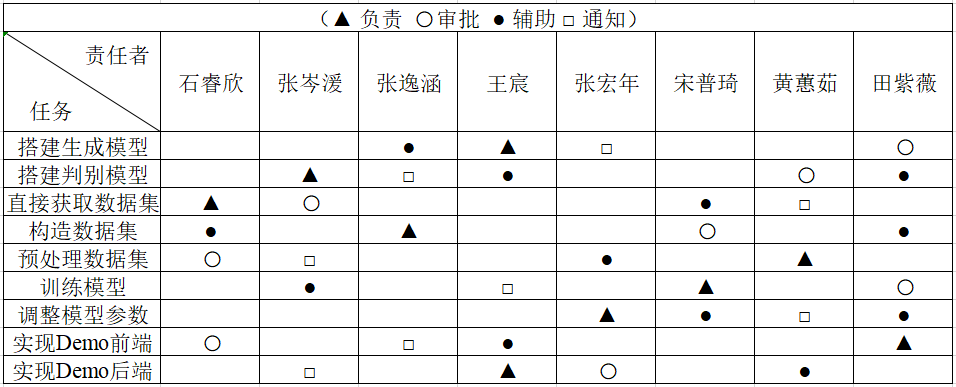
\includegraphics{1.png}
\caption{责任分配表}
\end{figure}

\hypertarget{ux9879ux76eeux8ba1ux5212ux5de5ux4f5cux5217ux8868}{%
\section{项目计划工作列表}\label{ux9879ux76eeux8ba1ux5212ux5de5ux4f5cux5217ux8868}}

见表3

\begin{table}
    \caption{工作列表}
    \begin{tabular}{|p{2.0cm}<{\centering}|p{2.0cm}<{\centering}|p{2.0cm}<{\centering}|p{2.0cm}<{\centering}|p{2.0cm}<{\centering}|}
    \hline
    任务编码 & 任务名称     & 紧前工作  & 时间估计(天) & 负责人 \\ \hline
    1    & 项目分析     & —     & 5       & 王宸  \\ \hline
    2    & 搭建生成模型   & 1     & 9       & 王宸  \\ \hline
    3    & 搭建判别模型   & 1     & 9       & 张岑湲 \\ \hline
    4    & 直接获取数据集  & 1     & 5       & 石睿欣 \\ \hline
    5    & 构造数据集    & 1     & 9       & 张逸涵 \\ \hline
    6    & 预处理数据集   & 4、5   & 6       & 黄蕙茹 \\ \hline
    7    & 训练模型     & 2、3、6 & 3       & 宋普琦 \\ \hline
    8    & 调整模型参数   & 7     & 5       & 张宏年 \\ \hline
    9    & 实现Demo前端 & 1     & 14      & 田紫薇 \\ \hline
    10   & 实现Demo后端 & 1     & 17      & 王宸  \\ \hline
    \end{tabular}
\end{table}

\hypertarget{ux9879ux76eeux7f51ux7edcux56fe}{%
\section{项目网络图}\label{ux9879ux76eeux7f51ux7edcux56fe}}

\begin{figure}
\centering
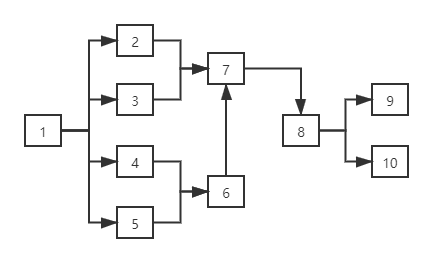
\includegraphics{2.png}
\caption{网络图}
\end{figure}

\hypertarget{ux7518ux7279ux56fe}{%
\section{甘特图}\label{ux7518ux7279ux56fe}}

\begin{figure}
\centering
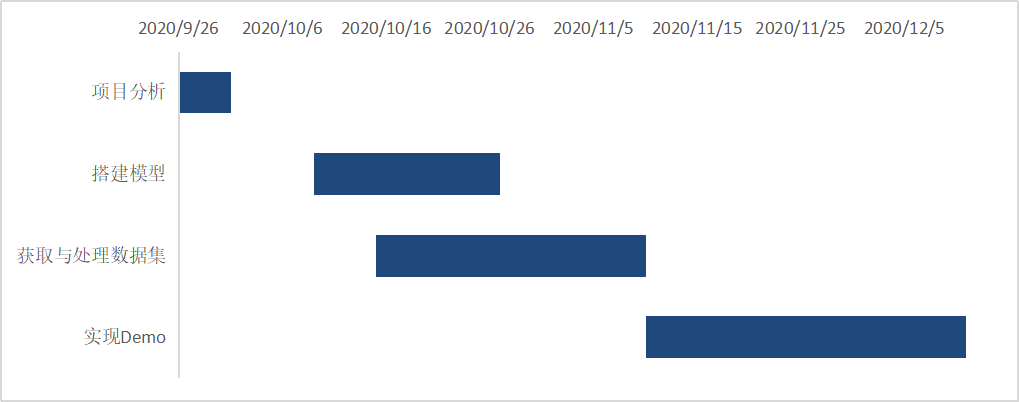
\includegraphics{3.png}
\caption{Gantt图}
\end{figure}

\hypertarget{pertux65f6ux95f4ux5206ux6790}{%
\section{PERT时间分析}\label{pertux65f6ux95f4ux5206ux6790}}

根据计划评审技术推测,

\end{document}
